\chapter{Hardware e Software}%
    \label{chp:hs}
	
	\section{Hardwares da Planta de Controle}
    	A planta possui uma eletrônica embarcada responsável por fazer a alimentação dos componentes, sensoriamento dos graus de liberdade, e atuação dos motores. Dua baterias são utilizadas para fornecer energia ao dispositivo. A integração do microprocessador com os componentes da planta, bem como dos componentes entre sí, pode ser vista no diagrama elétrico na Figura \ref{img:diagrama}.
    	
    	\begin{figure}[h]
            \centering
            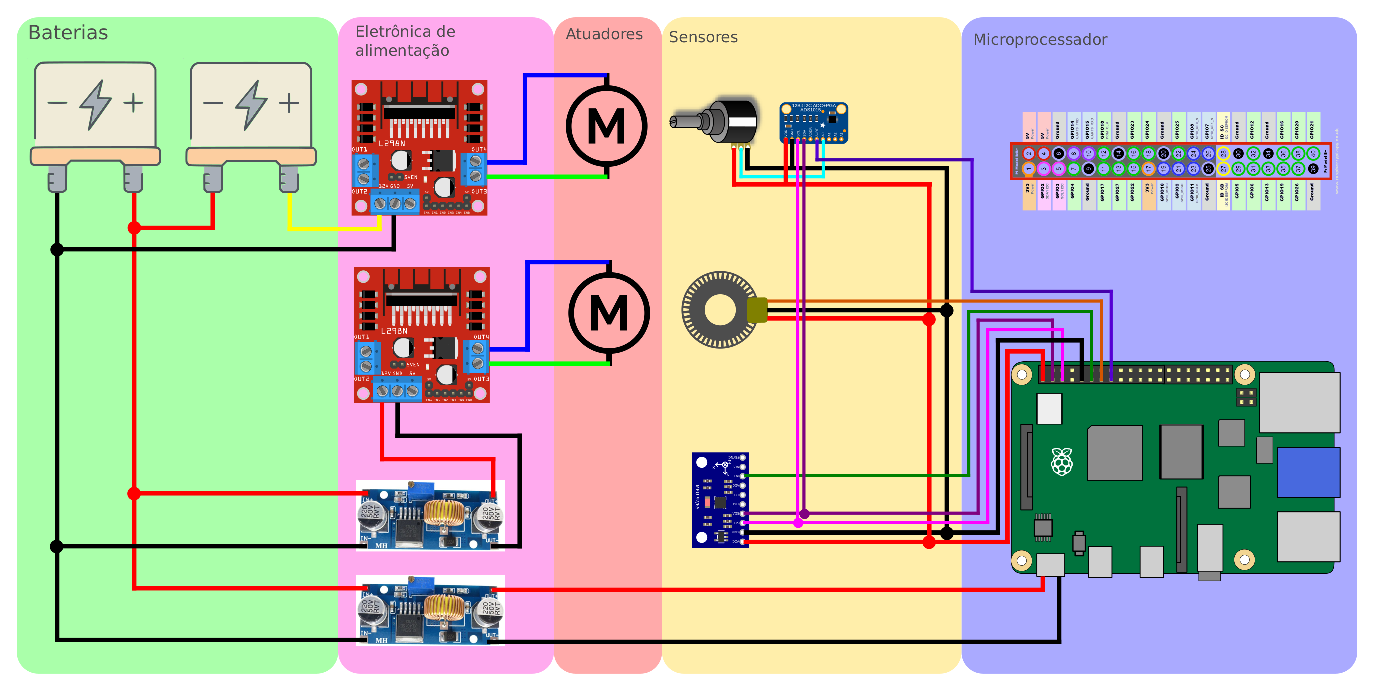
\includegraphics[width=\columnwidth]{Imagens/cap2/montagem3.eps}
            \caption{Diagrama elétrico da planta.}
            \label{img:diagrama}
        \end{figure}
        
        \subsection{Microprocessador}
    	    
    	    O microcontrolador proposto para a realização deste trabalho foi o Raspberry Pi 4 Model B. Ele possuí um processador \textit{Broadcom BCM2711} que possuí quatro núcleos \textit{Cortex-A72} rodando a uma frequência de $1.5 GHz$ cada, e possuem arquitetura \textit{ARM64}. Ele possuí um barramento de pinos que permite a conexão com sensores e outros dispositivos eletrônicos através de diversos protocolos, como \textit{PWM}, \textit{I2C}, \textit{SPI}, etc. A tensão de alimentação da placa é de $5V$.
    	
        	\begin{figure}[h]
                \centering
                \includegraphics[width=7cm]{Imagens/cap2/rasp2.jpg}
                %\caption{Raspberry Pi 4 com \textit{case} de proteção e resfriamento.}
                \caption{Raspberry Pi 4 model B.}
                \label{img:theta}
            \end{figure}
    	
    	    A \textit{GPIO} do \textit{Raspberry} trabalha com tensão $3.3V$, por isso os sensores serão alimentados com a mesma tensão. O \textit{Raspberry} fornece um pino de saída com essa tensão, que é usado para alimentar os sensores.
        
        \subsection{Sensores}
        
        	Para realizar o sensoriamento da inclinação da planta em relação a gravidade é usado o sensor inteligente \textit{MPU-9250}, que contém vários sensores embutidos: 3 Acelerômetros, 3 Giroscópios e 3 Magnetômetros, totalizando 9 graus de liberdade. Sendo que cada trio de sensores são perpendiculares entre si. Além disso ele possui um \textit{DMP (Digital Motion Processor)}, que é um microprocessador que realiza a fusão de sensores a fim de obter a orientação espacial do conjunto. Como o sensor é fixo em relação ao corpo da planta, é possível obter a inclinação em relação a gravidade através da orientação espacial que o sensor fornece. Uma foto do sensor pode ser vista na Figura \ref{img:mpu}.
        	
        	\begin{figure}[h]
                \centering
                \includegraphics[width=4cm]{Imagens/cap2/mpu.png}
                \caption{Foto do sensor \textit{MPU-9250}}
                \label{img:mpu}
            \end{figure}
            
        	O eixo de direção da roda dianteira possui um servo motor \textit{TowerPro MG995} acoplado, composto por um motor, uma redução de engrenagens, e um potenciômetro integrado. O potenciômetro tem 3 vias e uma resistência interna de $10k$. Originalmente este servo vem com um uma placa de circuito integrado que realiza a comunicação com um micro-controlador e o controle do eixo de saída, mas tal placa foi retirada para o controle ser feito diretamente pelo microcontrolador. O potenciômetro, por sua vez, é conectado a um conversor analógico digital \textit{Ads1115} que converte a tensão de saída em uma faixa de 16 bits, e envia a leitura para o microcontrolador.
    	
        	\begin{figure}[h]
                \centering
                \includegraphics[width=4cm]{Imagens/cap2/995.png}
                \caption{Foto do servomotor \textit{TowerPro MG995}.}
                \label{img:theta}
            \end{figure}
            
            \begin{figure}[h]
                \centering
                \includegraphics[width=4cm]{Imagens/cap2/ads.png}
                \caption{Foto do conversor analógico digital \textit{Ads1115}.}
                \label{img:theta}
            \end{figure}
            
        	O sensoriamento da velocidade tangencial é realizado por um encoder óptico \textit{OPB-991T51}. Ele é composto por um LED infravermelho, um foto-transistor, e um disco com orifícios. O LED fica alinhado com o foto-transistor, que dependendo da posição angular do disco, impede ou não a passagem do infravermelho. Quando há a passagem de luz o foto-transistor fecha circuito elétrico, e vice-versa. Como o disco do encoder está acoplado a roda traseira, partindo do pressuposto que a roda gira apenas em um sentido, é possível saber aproximadamente quantos graus a roda girou através do sinal elétrico. Logo, é possível um microcontrolador calcular a velocidade tangencial dividindo a variação angular pela variação de tempo. Uma foto do conjunto do encoder pode ser vista na Figura \ref{img:encoder},
        	
        	\begin{figure}[h]
                \centering
                \includegraphics[width=8cm]{Imagens/cap2/foto-encoder.jpg}
                \caption{Foto da vista lateral esquerda da planta - Encoder Óptico \textit{OPB-991T51}.}
                \label{img:encoder}
            \end{figure}
        
        \subsection{Atuadores}
        
    	    A roda traseira tem também um atuador acoplado a ela por intermédio de uma polia-correia. O motor é de corrente continua de ímã permanente, como explicado na sessão \ref{sec:motorcc} e este pode receber uma tensão máxima de $24V$. Os outros parâmetros referentes ao motor, bem como da polia-correia, serão fornecidos na sessão \ref{sec:modelagemvelocidade}. Uma foto do motor acoplado a polia pode ser visto na Figura \ref{img:motor-polia}.
    	
        	\begin{figure}[h]
                \centering
                \includegraphics[width=8cm]{Imagens/cap2/foto-motor-polia.jpg}
                \caption{Foto da vista lateral direita da planta - Motor e Polia.}
                \label{img:motor-polia}
            \end{figure}
    	    
    	    O motor do servo motor acoplado ao eixo de direção, de acordo com a fabricante, suporta uma tensão máxima de $7,2V$. Novamente, os outros parâmetros referentes ao motor, bem como da redução, serão fornecidos na sessão \ref{sec:modelagemvangulo}.
    	
    	\subsection{Eletrônica de alimentação e Baterias}
    	    
    	    Ambos motores são alimentados por intermédio de uma ponte H \textit{LN298} para cada. Elas são responsável por receber um sinal \textit{PWM} cada do microcontrolador, e aplicar esse sinal em seu respectivo motor.
    	
        	\begin{figure}[h]
                \centering
                \includegraphics[width=5cm]{Imagens/cap2/ln298.png}
                \caption{Foto da ponte H \textit{LN298}}
                \label{img:theta}
            \end{figure}
        
    	    As baterias que alimentam a planta são de polímero de lítio, com tensão nominal de $12,6V$. Cada célula de carga trabalha com uma tensão que varia de $3.5V$ quando descarregadas a $4,2V$ quando em carga máxima. Como cada bateria possuí 3 células, a tensão de trabalho de cada bateria varia de $12,6V$ a $10,5V$. As duas estão associadas em série, totalizando um tensão aproximada de $24V$, tendo disponível o terminal intermediário entre elas com tensão de $12V$.
    	
        	\begin{figure}[h]
                \centering
                \includegraphics[width=5cm]{Imagens/cap2/bateria.jpg}
                \caption{Foto do tipo de bateria de polímero de lítio utilizado.}
                \label{img:theta}
            \end{figure}
    	    
    	   Como alguns dispositivos tem tensão diferente da bateria, faz-se necessário abaixar essa tesão para determinados dispositivos. Para isso vem acoplados na planta dois conversores de tensão \textit{Step-down} \textit{Xl4015} que convertem a tensão da bateria para o valor necessário. O primeiro é ajustado em $7V$ para alimentar a ponte-H que alimenta o servomotor, enquanto a ponte h que alimenta o motor traseiro recebe tensão direta vinda da bateria. E o outro conversor é ajustado para uma saída de $5V$ para alimentar o microprocessador.
    	
        	\begin{figure}[h]
                \centering
                \includegraphics[width=4cm]{Imagens/cap2/xl.jpg}
                \caption{Foto do conversor de tensão \textit{Xl4015}.}
                \label{img:theta}
            \end{figure}
        
        \subsection{Gamepad}
        
            Como a planta de controle é móvel, é necessário um emissor de sinais sem fio, a fim de permitir enviar comandos e valores de referencia para a planta, como iniciar ou parar os controladores e a referência do sistema de equilíbrio. Para isso foi escolhido o \textit{DualShock 4} que é o gamepad do videogame \textit{PlayStation 4} da marca \textit{Sony}, devido que o kernel do Linux já tem os drivers de comunicação para este gamepad, já existem bibliotecas de código aberto disponíveis para realizar a comunicação com esse controle em algumas linguagens de programação, e o preço acessível quando importado direto da China.
            
            \begin{figure}[h]
                \centering
                \includegraphics[width=4cm]{Imagens/cap2/DualShock_4.jpg}
                \caption{Foto do Gamepad \textit{DualShock 4}.}
                \label{img:ds4}
            \end{figure}
            
            Este gamepad possuí suporte para o protocolo de comunicação \textit{Bluetooth 2.1 + EDR}, que através dele é realizada a comunicação com Raspberry Pi 4. Como entrada possui 2 manetes analógicas de 2 eixos cada, 2 gatilhos analógicos, 12 botões digitais, 4 botões direcionais digitais, 1 touchpad capacitivo de 2 pontos de contato, 3 eixos acelerômetros e 3 eixos giroscópios.
            
            
    \section{Softwares da Planta de Controle}
        
        O Raspberry Pi 4 tem um sistema operacional oficial baseado em linux chamado \textit{Raspberry Pi OS}, que é basicamente um sistema operacional \textit{Debian} com os repositórios de software da própria raspberry e com uma interface gráfica que é uma remasterização da interface \textit{LXDE} chamada \textit{PIXEL}. É possível instalar outros sistemas operacionais, entretanto foi optado instalar o sistema operacional oficial devido que, além dele já vir otimizado para o hardware, vem instaladas bibliotecas que auxiliam o desenvolvimento de software em varias linguagens de programação, como Pyhton e C++.
        
        A linguagem de programação escolhida para realizar o desenvolvimento dos softwares da planta que rodarão no Raspberry foi Python na sua versão 3, devido que existem varias bibliotecas de código aberto para os sensores disponíveis nessa linguagem e devido à facilidade de realizar a programação devido sua sintaxe simples. Mas devido a motivos que serão visto na subsessão \ref{}, foi necessário desenvolver um novo programa em Python, aproveitando o que foi desenvolvido anteriormente, mas desenvolvendo os códigos dos controladores em C++ e realizando a comunicação entre os dois processos.
        
        
    \section{Software MotinhaPi}
        
        Inicialmente foi desenvolvido um software chamado MotinhaPi, visando cumprir varias funções ao mesmo tempo, devendo cada funcionalidade ser ativada ou não pelo gamepad:
        \begin{itemize}
            \item Operar suas funcionalidades conforme recebe comandos do gamepad.
            \item Realizar a aquisição de dados dos sensores e atuadores em tempo real e salvando-a em um arquivo.
            \item Executar sinais em malha aberta oriundos do gamepad.
            \item Executar sinais salvos na memória do microprocessador.
            \item Receber o sinal de referência dos controladores oriundos do gamepad.
            \item Executar os controladores de cada sistema a uma taxa de amostragem específica.
        \end{itemize}
        
        Quando o botão triangulo do gamepad é pressionado, o programa ativa uma função que realiza a aquisição de dados dos sensores e atuadores, e vai salvando essa aquisição em um arquivo para os dados serem utilizados para a analise em um programa adequado, como MATLAB Matworks, bem como serem usados os sinais em simulações no Simulink, e também para gerar gráficos da resposta do sistema.
        
        \subsection{Função malha aberta para identificação - Sinal oriundo do gamepad}
        
            Para realizar a identificação do sistema em malha aberta é necessário realizar a análise da entrada e da saída do sistema, ou seja, a leitura dos sensores e atuadores. Para isso foi desenvolvida uma função de envio de sinais em malha aberta utilizando dispositivos do gamepad. Quando pressionado o botão L3 por exemplo, ele entra no modo malha aberta do sistema de tração, logo as setas direcionais são programadas para cada uma das 4 representar uma amplitude diferente do sinal do atuador, conforme tabela abaixo, e a manete analógica esquerda no sentido vertical varia o sinal do atuador de $+100\%$ até $-100\%$.
            
            \begin{table}[]
                \begin{tabular}{lll}
                    Botão/Manete          & Amplitude (V) & Obs.                                             \\
                    Pressionar Manete L3  & 0             & Ativa malha aberta para o sistema de velocidade. \\
                    Direcional Esquerda   & 0             & Desligado.                                       \\
                    Direcional Direita    & 12            & Ponto de Operação (P.O.).                        \\
                    Direcional Cima       & 13,2          & P.O. + 10\%.                                     \\
                    Direcional Baixo      & 10,8          & P.O. - 10\%.                                     \\
                    Manete L3 Vertical    & +24 / -24     & Varia analogicamente no intervalo.               \\
                    Maneta L3 Horizontal  & *             & Sem função.                                     
                \end{tabular}
            \end{table}
            
            Desta forma fica muito fácil gerar os sinais de entrada para realizar o experimento identificação do sistema, bastando realizar comandos pelo gamepad. É também seguro porque permite o controle da planta a distancia, bem como a interrupção imediata do teste, além da funcionalidade extra de frear a planta em caso de emergência, evitando acidentes, já que a mesma pode atingir velocidade superiores a $20Km/h$.
        
        \subsection{Função malha aberta para identificação - Sinal oriundo da memória}
        
            Uma outra estrategia para enviar os sinais para o atuador e realizar o experimento para identificação de um sistema é enviar um sinal pré-programado, com formato mais complexo, como por exemplo o sinal \textit{sweepsine} que é basicamente uma senoide com frequência variante no tempo.
            
            Enviar o sinal pré-programado é interessante pois alguns sistemas apresentam limites físicos para a saída, como o sistema de direção por exemplo, onde existe uma trava no servomotor limitando o movimento em $\pm 180\°$, e atingir essa trava força as engrenagens podendo quebrar o equipamento. É possível enviar um sinal ao atuador de certa forma que a saída não sature, tendo como característica um sinal de média $0$, por exemplo.
            
            Para envio deste sinal foi programado o botão L1. Quando pressionado ele ativa a thread, realizando a leitura do sinal na memoria e imediatamente passando a enviar o sinal para o atuador. Antes de ativar essa funcionalidade, deve-se ser pressionado o botão triangulo para ativar a thread que salva a leitura dos sensores e atuadores em um arquivo.
        
        \subsection{Drivers de comunicação com sensores e atuadores}
            RPi.GPIO, busio
            pyPS4Controller, adafruit_ads1x15, rpi_hardware_pwm
            
        \subsection{Gerenciamento da taxa de amostragem}
            
            time, threading
        
        \subsection{Função malha fechada}
        
            Como são três sistemas de malha fechada, foi definido um botão para ativar cada, sendo:
            \begin{itemize}
                \item Botão X: Sistema de controle de velocidade
                \item Botão O: Sistema de controle de direção (independente)
                \item Botão Quadrado: Sistema de controle de inclinação e direção
            \end{itemize}
            
            Quando o botão X é pressionado é iniciado a thread responsável por receber a referência de velocidade do gamepad, calcular a velocidade pelo sensor, calcular o sinal de erro, o sinal de controle, e enviar para o atuador. A referência vem da manete analógica L3 vertical.
            
            Quando o botão O é pressionado é iniciado a thread responsável por receber a referência de posição angular do gamepad, calcular a posição angular da direção pelo sensor, calcular o sinal de erro, o sinal de controle, e enviar para o atuador. A referência vem da manete analógica R3 horizontal.
            
            Quando o botão Quadrado é pressionado é iniciado a thread responsável por receber a referência de inclinação do gamepad, calcular a posição angular da planta pelo sensor, calcular o sinal de erro, o sinal de controle, e enviar o sinal de controle como referencia para o controlador de direção, que por sua vez irá repedir o processo do parágrafo anterior. A referência de inclinação também vem da manete analógica R3 horizontal.
            
            Não se deve iniciar as duas threads juntas referentes ao botão O e quadrado. Ou se controla a direção independentemente, útil para coletar dados do sistema em malha fechada, ou se controla a inclinação da planta e deixa a referência de direção a cargo do controlador da planta.
            
        \subsection{Problemas com Python}
        
            Taxa de amostragem 
        
    \section{Software MotinhaPiCpp}
    
        O software MotinhaPiCpp é uma versão nova do software anterior, cuja principal diferença é que os controladores são executados separados em uma thread escrita na linguagem em C++. A thread principal do programa, escrita em Pyhton, se comunica com as threads dos controladores enviado as referências para o mesmo, oriundas do gamepad. 
        
        \subsection{Comunicação entre threads}
            Entrada e saída padrão SDTIN SDTOUT
        
        \subsection{Taxa de amostragem obtida}
            
        
    \section{Simulações e tratamento de dados}
        
        Os dados gerados pelos softwares MotinhaPi e MotinhaPiCpp salvos em arquivo de texto, são importados para o MATLAB para tratar os dados, realizar a identificação do sistema e as simulações.
        